% ==========================================================================
%  Section 10 -- Scope, boundaries, and the wider programme.  Owner: W09.
%  Frozen label: sec:scope.  Only W09 may \begin{figure}[t]
\centering
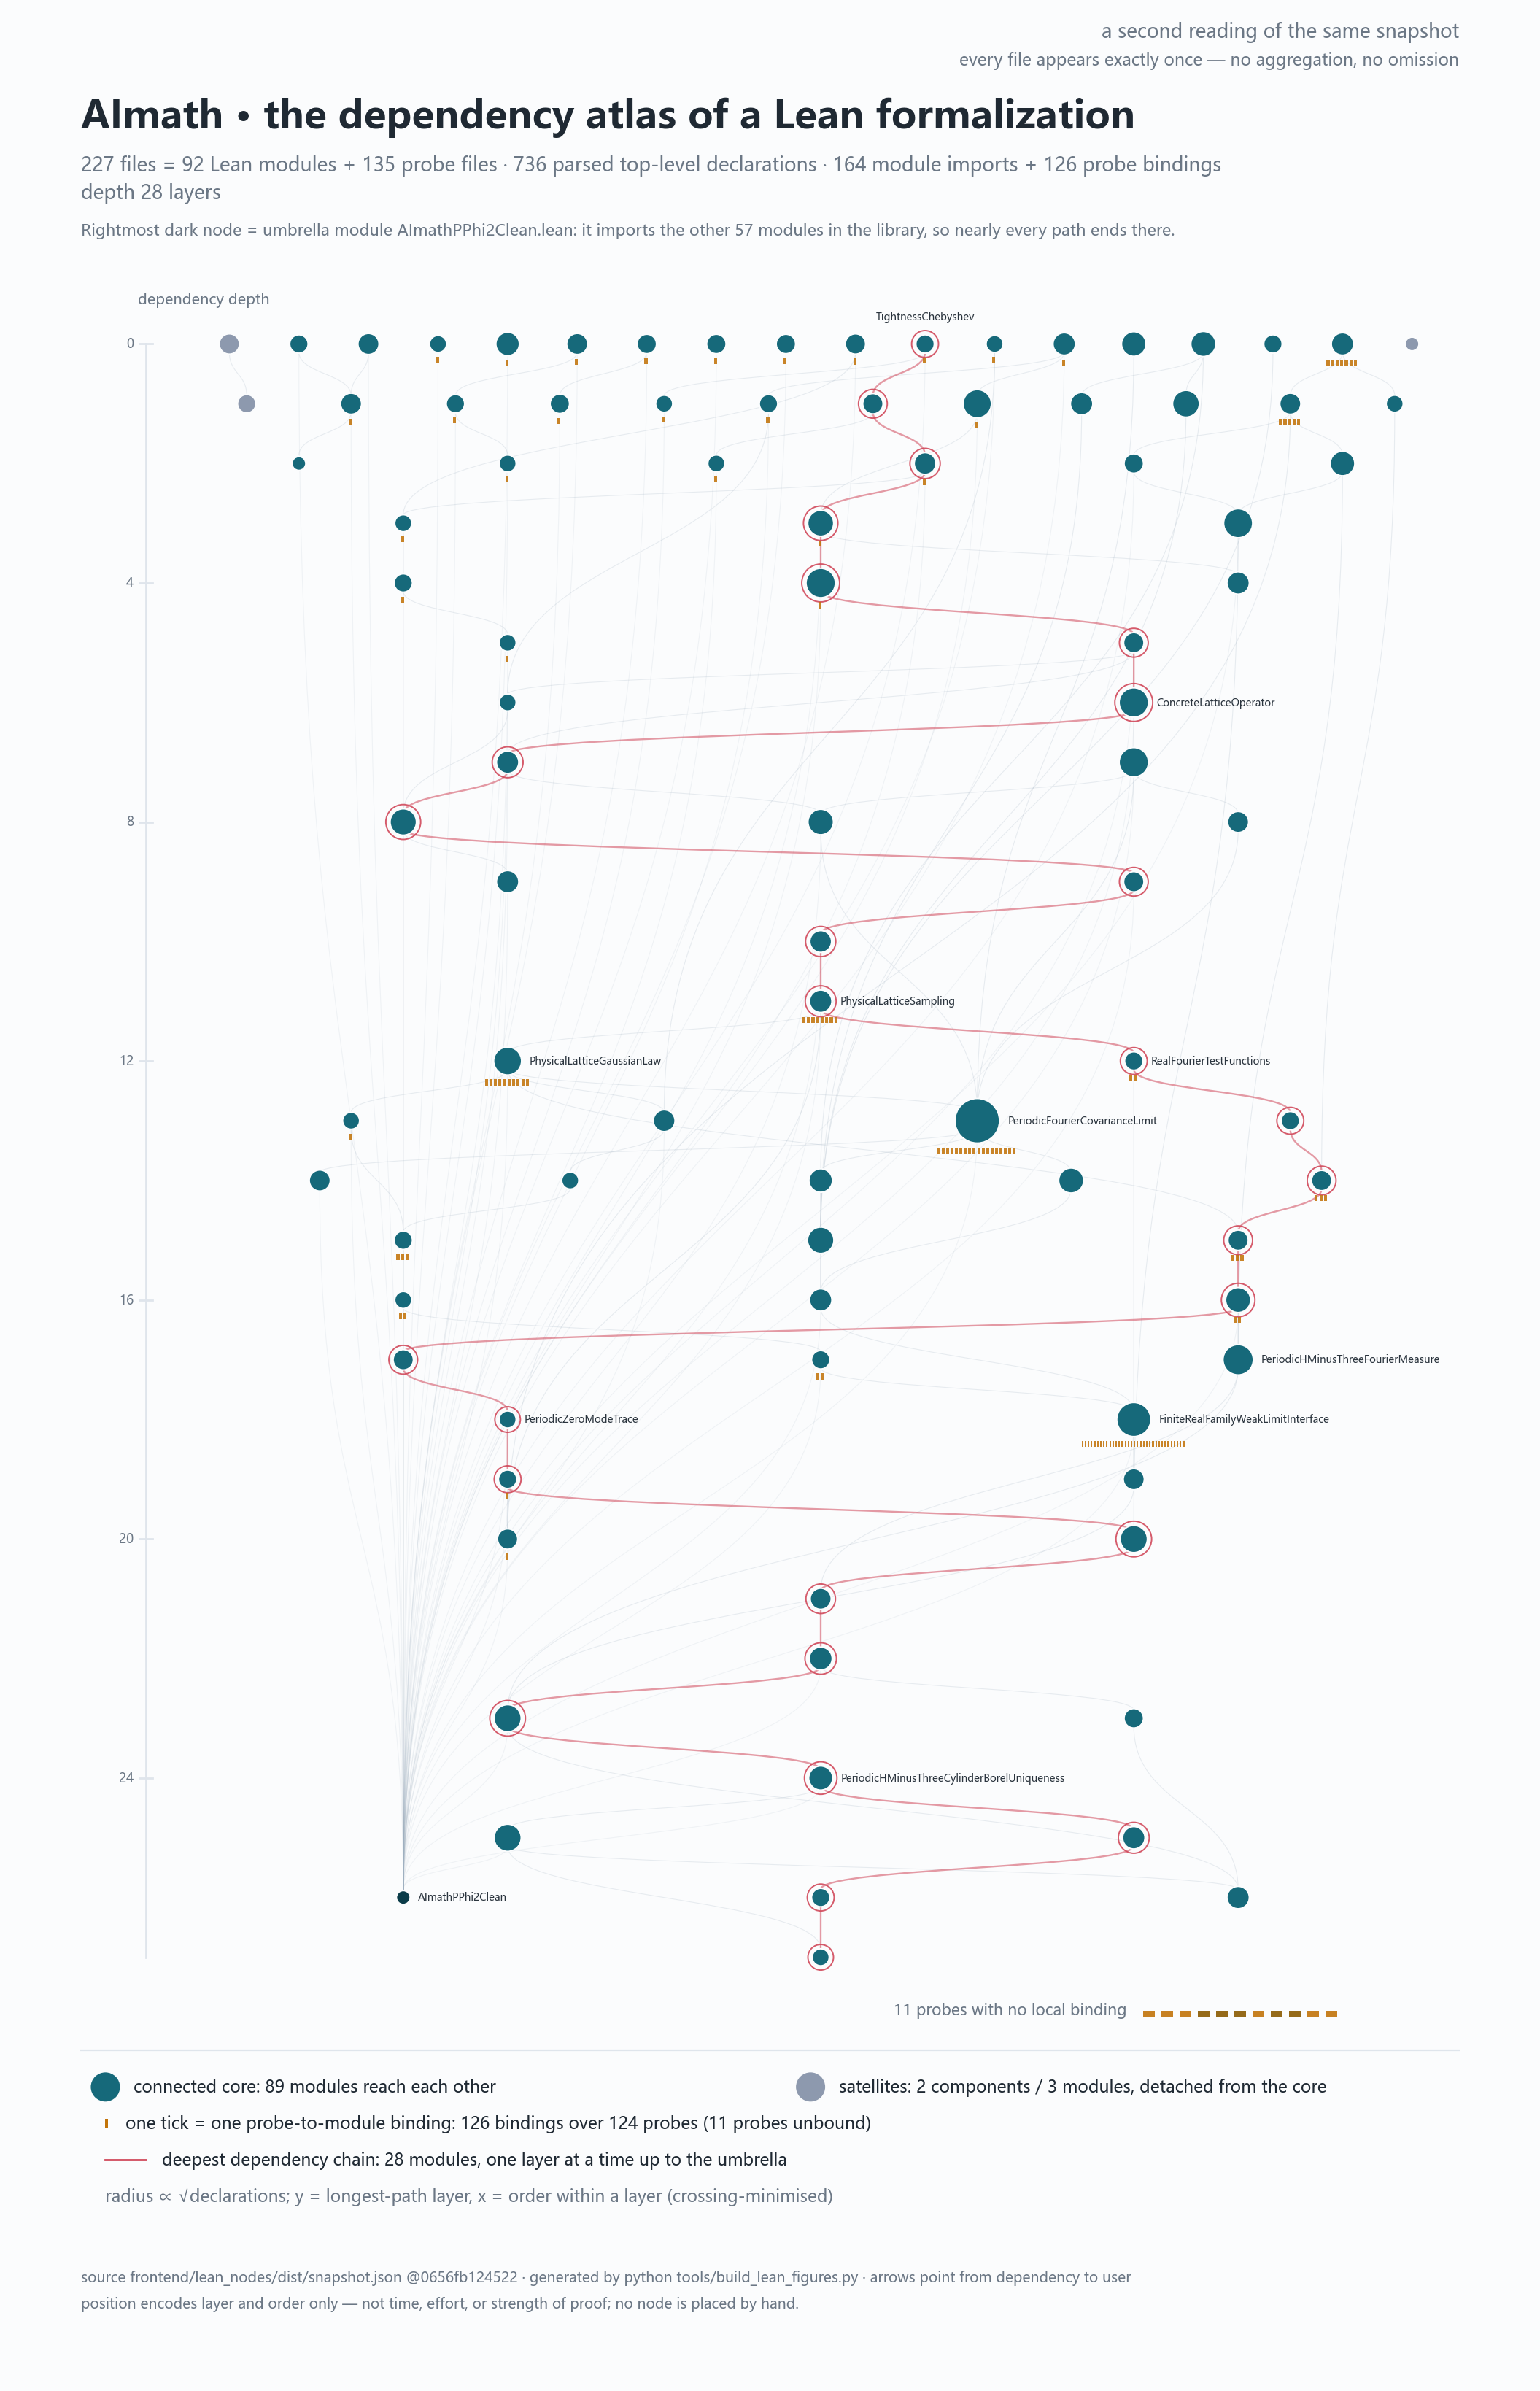
\includegraphics[width=0.62\linewidth]{figures/lean_atlas_en_portrait.png}
\caption{Dependency atlas of the Lean development. Each node is a module and each edge a declaration dependency. The atlas is a snapshot of a slightly wider tree than the package of \cref{sec:lean-overview}: it reports $92$ modules and $135$ probe files against the package's \NumCleanModules{} and \NumAuditProbes, and the figure's own legend identifies the three extra modules as satellites detached from the core rather than as part of it. The dense core the atlas names is the package. The surrounding directory of \cref{sec:lean-overview} is much larger than either count --- it holds \NumRootFiles{} further modules --- and none of it is drawn here. The figure is therefore best read as a picture of where the reported chain sits inside the tree that was measured, not as evidence about anything outside that chain.}
\label{fig:atlas}
\end{figure}
.
%
%  Each exclusion is stated with the reason it is a boundary of the statement
%  rather than a missing step: GAP R3 is item 1, GAP R4 item 3, GAP R7 item 4,
%  and the dimension restriction is item 5.
%
%  No priority claim is made, and no work is promised.  The citations are for
%  position only; the four structural points at the end are checkable in the
%  text and are not comparative.
%
%  Appendices are named in words rather than with \cref: their labels live in
%  main.tex, which the paper gate does not scan (same convention as W10).
% ==========================================================================
\section{Scope, boundaries, and the wider programme}\label{sec:scope}

Let $L>0$ and $m>0$.  \Cref{thm:main} proves that the finite-source Fourier
pushforwards $\mu_N$ of the fixed-volume lattice Gaussian laws converge weakly, as
a whole sequence, to the single Borel probability measure on the carrier
$\mathcal C=\HL{3}$ that their finite Fourier marginals determine. Its hypotheses
are proved in the same chain and not assumed: the tightness of the family
(\cref{thm:tightness}), with the uniform $\HL{2}$ moment behind it, and the limits
of the finite-marginal laws (\cref{thm:finite-family}), whose target is the paired
cosine and sine Gaussian law of the periodic resolvent.  Separately,
\cref{thm:covariance-limit} proves the analytic limit: the covariance integrals of
the physical lattice laws $\mu^{\mathrm{GJ}}_N$ converge to the pairing with the
resolvent of \cref{lem:resolvent}.  This section does the
opposite job.  It records what neither statement asserts, places what they do
assert among the branches of the programme, and points to the machine-checked
layer.

\subsection{What the paper does not assert}

Five boundary statements belong in the body rather than in a footnote: a reader who
supplies one of them from context would read the paper as claiming more than it
proves.  Each carries the reason it is a boundary of the statement, not a gap in
its proof.

\begin{enumerate}
\item \emph{What converges is the law of the Fourier coefficients.}  The
  sequence in \cref{thm:main} is $\mu_N=(L_N)_*\,\mu^{\mathrm{GJ}}_N$ of
  \cref{def:finite-source-lift}, and \cref{lem:lift-representative} identifies
  this as the law of a Borel carrier-valued map of the lattice Gaussian field.
  So the theorem does concern the lattice field laws; what it does not touch is
  any total lift specified independently of $L_N$ --- in particular the
  series-defined lift of the development, which carries its own measurability
  input (\cref{rem:lift-development}) --- and it says nothing about the field as
  a distribution on $\Torus$.  ``The lattice field laws converge'' is therefore
  asserted in the sense of the law of the coefficient sequence, which is the
  sense in which $\mu_N$ is a measure on $\mathcal C$ at all.
\item \emph{No identification with a distribution-defined Sobolev space, and no
  Laplacian domain theorem.}  The carrier is the explicit weighted $\ell^2$
  space of \cref{def:carrier-hminus3}, and \cref{prop:completion} is a statement
  about it: isometrically $\ell^2$, with $\HL{2}$ sitting inside continuously.
  The paper does not assert that $\mathcal C$ agrees with a Sobolev space of
  distributions defined independently of it, and it proves no strong domain
  theorem for an unbounded Laplacian.  Every estimate here is a weighted sum over
  modes, and no step is taken over from such an identification.
\item \emph{No covariance operator on the carrier, and no operator-level
  Gaussianity.}  The resolvent $R$ of \cref{lem:resolvent} is constructed on the
  $L^2$ space of the torus, not on $\mathcal C$, and no covariance operator is
  constructed on $\mathcal C$ here.  What is proved is the marginal statement of
  \cref{thm:main}(ii): for each finite tuple $F$ of modes, $(\Pi_F)_*\mu_{\mathrm{free}}$
  is the paired cosine and sine Gaussian law of \cref{thm:finite-family}.  Read
  as an operator statement, the proposition that $\mu_{\mathrm{free}}$ is the
  Gaussian measure whose covariance operator is $(m^2-\Delta)^{-1}$ is therefore
  not asserted.  A reader who wants it must either construct the operator on the
  carrier or use cylinder determination, since the cylinders generate the Borel
  sigma algebra (\cref{thm:cylinder-borel}) and the marginals determine the
  measure (\cref{thm:cylinder-uniqueness}).  It is listed here because it is a
  step this paper does not take.
\item \emph{No rate, no exponential tail, no modulus of continuity.}  Tightness
  (\cref{thm:tightness}) is Markov's inequality applied to the single first
  moment of \cref{thm:uniform-moment}, plus compactness of $\HL{2}$ sublevel
  sets in the weaker topology (\cref{thm:compact-tail}).  No exponential moment
  and no layer-cake argument enters, so no rate in $N$, no exponential bound on
  tail probabilities and no modulus of continuity for $\mu_{\mathrm{free}}$ is
  asserted.  A second moment of the norm is what \cref{ext:prokhorov} consumes through tightness, and nothing
  more.
\item \emph{The measure limit is two-dimensional.}  The mode lattice $\Z^2$, the
  weights $w_2,w_3$, the cylinder maps, the carrier and the law sequence are all
  two-dimensional, so \cref{thm:main} is a theorem about the two-dimensional
  carrier, and no dimensional generalisation of that carrier is claimed
  (\cref{rem:dimension}).  The covariance limit is the one statement whose
  source and machine-checked versions are registered for a general dimension
  $d$; Part~I writes the two-dimensional case that \cref{sec:setting} fixes.
  Nothing here says what becomes of the weights, the trace constant or the
  compact tail at $d\neq2$.
\end{enumerate}

\subsection{Where the result sits in the programme}

This paper is one step of one branch of a programme, and three other branches of
the same project are outside it.  Each is named so that a reader knows what this
paper is not about; none is evaluated, and nothing is promised.

\begin{itemize}
\item \emph{The free scalar theory in four dimensions} is the free massive
  Euclidean field on $\R^4$: the Gaussian measure on a space of distributions,
  its covariance, the Osterwalder--Schrader axioms for it, and the physics
  reconstructed from them.  This paper does not touch it; nothing here is stated
  on $\R^4$ or at infinite volume.
\item \emph{The interacting two-dimensional theory} is the $P(\varphi)_2$ model
  \cite{gjs1974}: interacting finite-volume laws, their ultraviolet limit at
  fixed volume, the axiom verification, and the mass gap.  This paper does not
  touch it; the laws whose covariance limit is \cref{thm:covariance-limit} are
  Gaussian at every mesh size.
\item \emph{The QED programme} is the non-perturbative construction of
  four-dimensional quantum electrodynamics, with its reconstruction and its
  physical content.  This paper does not touch it; no gauge-theoretic object
  occurs in the argument.
\end{itemize}

\begin{figure}[t]
\centering
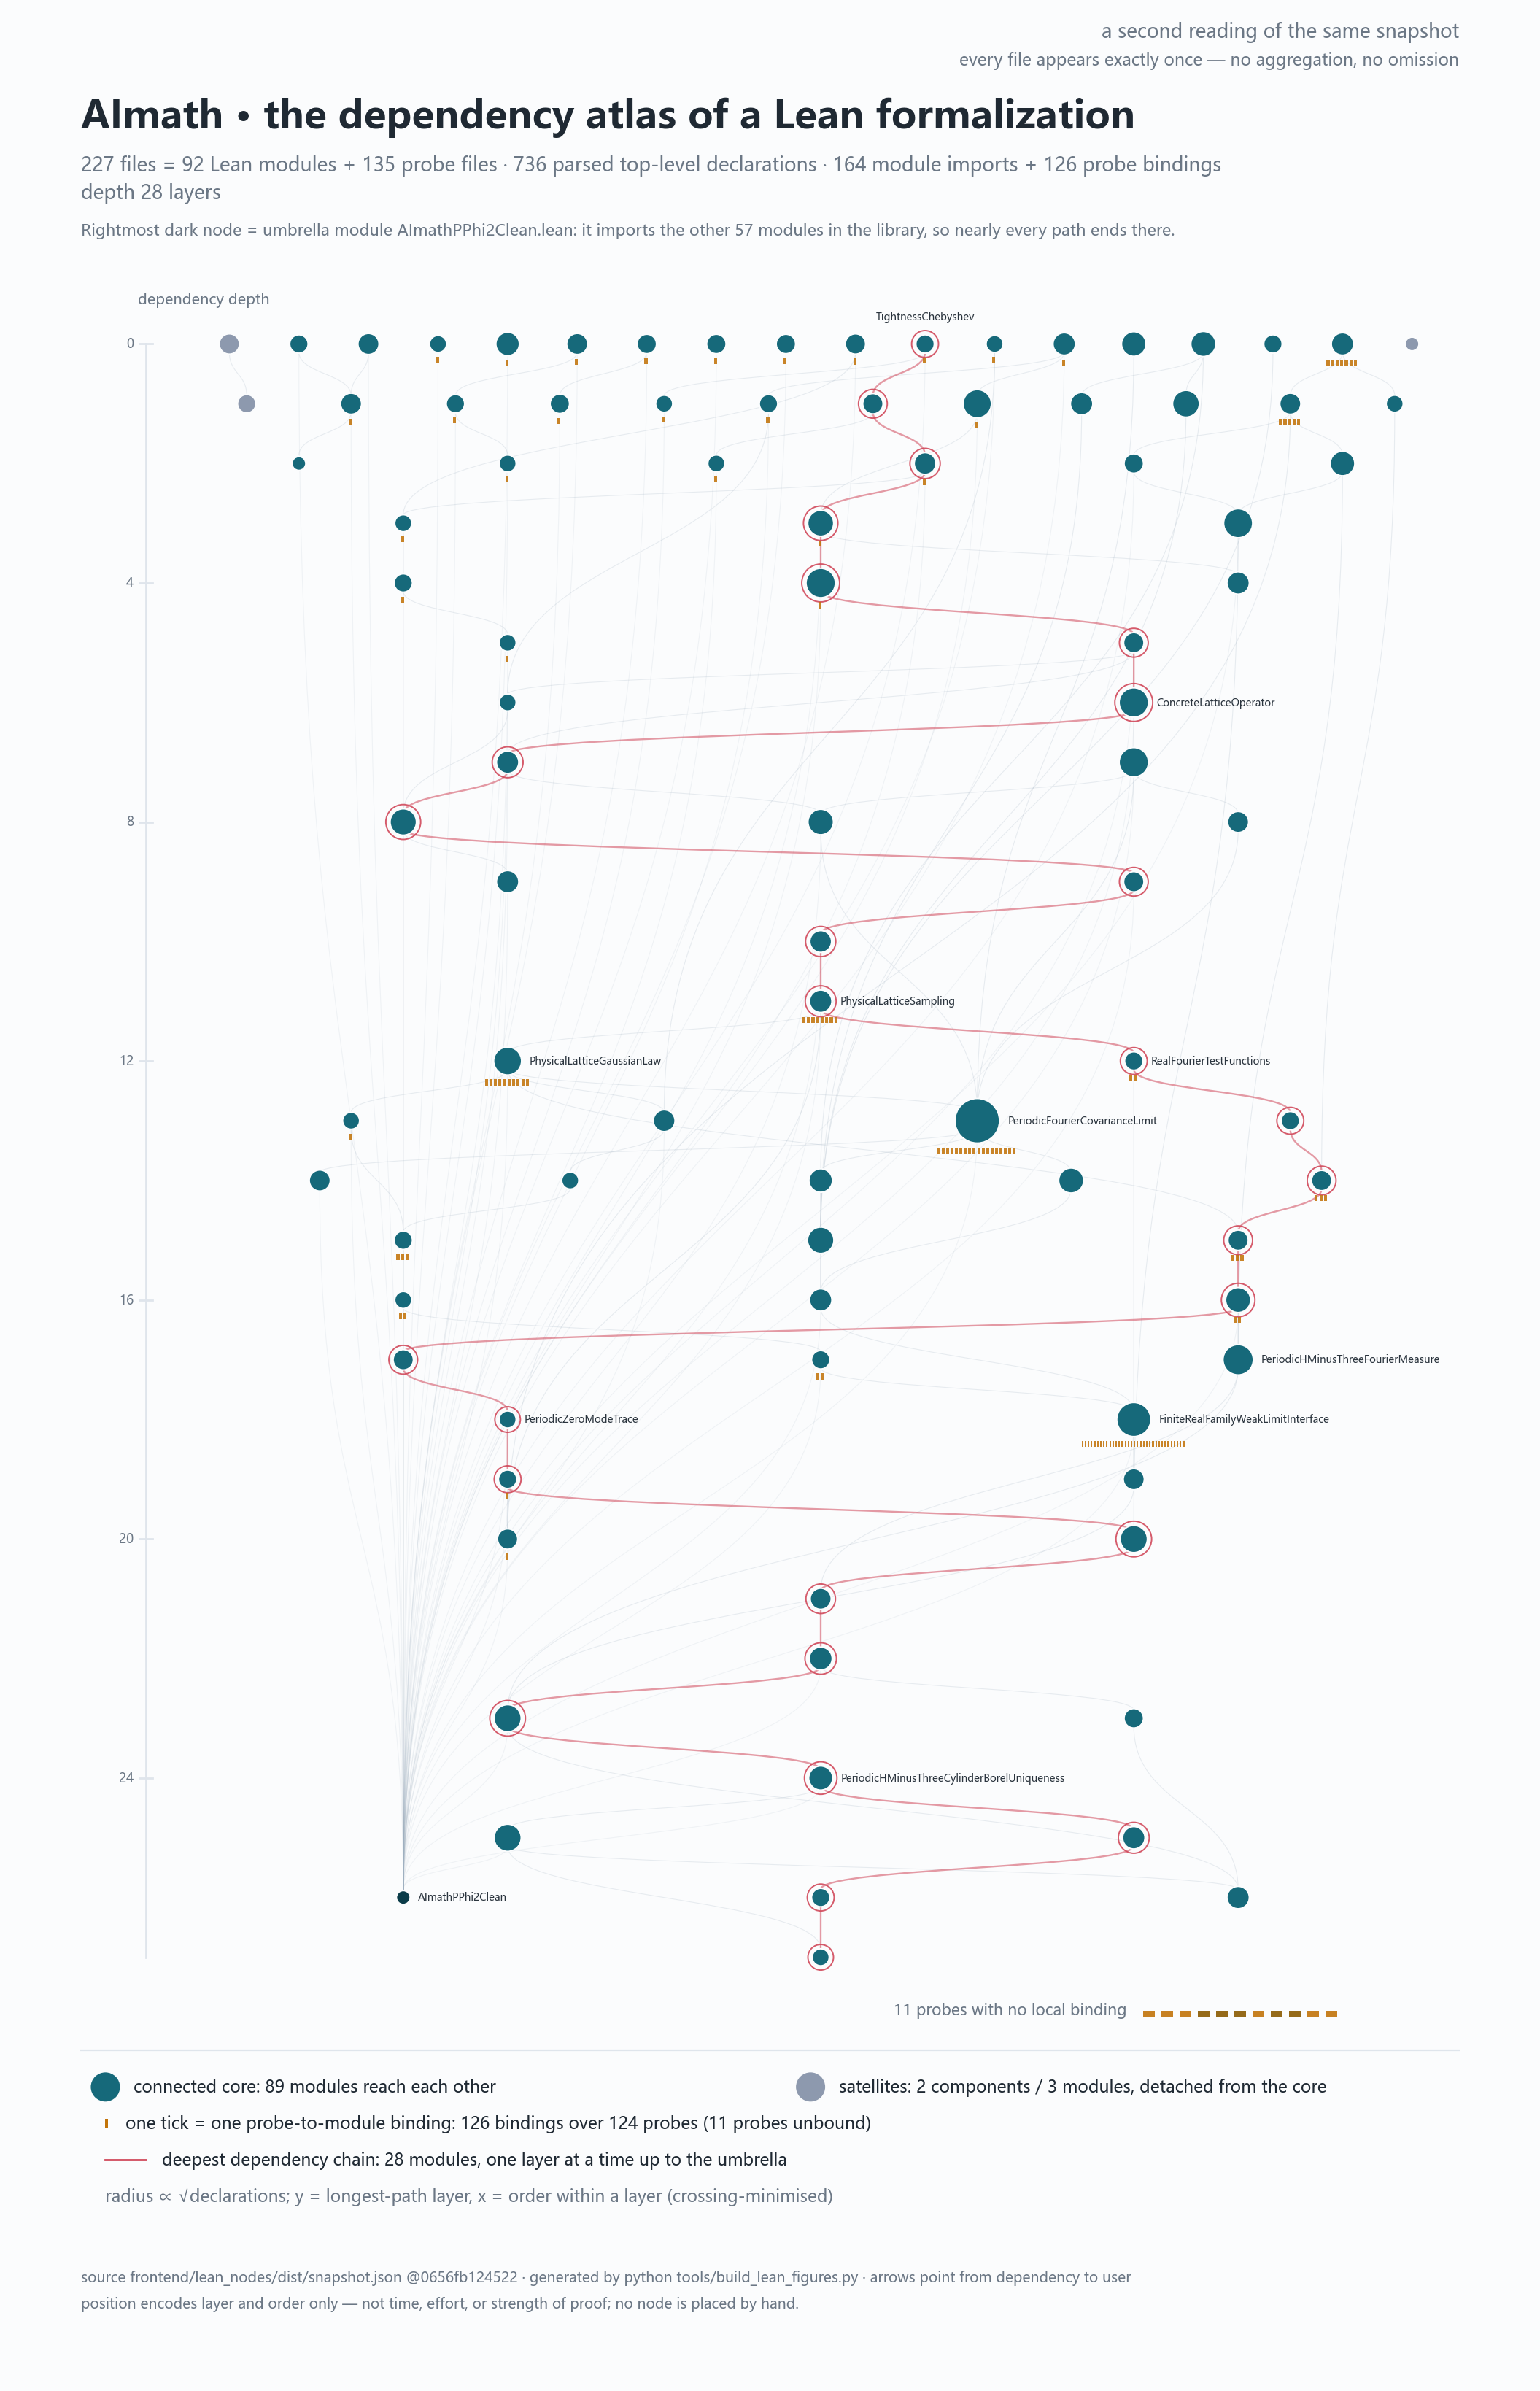
\includegraphics[width=0.62\linewidth]{figures/lean_atlas_en_portrait.png}
\caption{Dependency atlas of the Lean development. Each node is a module and each edge a declaration dependency. The atlas is a snapshot of a slightly wider tree than the package of \cref{sec:lean-overview}: it reports $92$ modules and $135$ probe files against the package's \NumCleanModules{} and \NumAuditProbes, and the figure's own legend identifies the three extra modules as satellites detached from the core rather than as part of it. The dense core the atlas names is the package. The surrounding directory of \cref{sec:lean-overview} is much larger than either count --- it holds \NumRootFiles{} further modules --- and none of it is drawn here. The figure is therefore best read as a picture of where the reported chain sits inside the tree that was measured, not as evidence about anything outside that chain.}
\label{fig:atlas}
\end{figure}


The atlas of \cref{fig:atlas} is a module-level dependency graph of the wider
Lean development of the project: its nodes are modules of that development as a
whole, not of the package this paper reports, and its edges are declaration
dependencies.  The package that Part~II reports is one cluster inside the atlas,
and the layers tabulated in \cref{sec:lean-overview} are the interior of that
cluster.

\subsection{Relation to the literature}

\NumCitedWorks{} works are cited in this paper, in two capacities that must not be
confused.  Four support a standard fact where it is used -- the Riesz
representation behind \cref{lem:resolvent}, the Prokhorov extraction of
\cref{ext:prokhorov}, the convergence of Gaussian laws with convergent
covariance matrices in \cref{thm:finite-family}, and the definition of weak
convergence on a metric space in \cref{rem:topology} -- and each is cited at that
point rather than here.  The remaining eight support nothing: they are cited
for position, and each of the following relations is a position, not a
dependency.  Seven of them are named below; the eighth, \cite{gjs1974}, is
named among the exclusions above.

\begin{itemize}
\item \cite{ossier1973,ossier1975} state the axioms: the properties
  (analyticity, reflection positivity, Euclidean invariance, clustering and
  regularity) that a Euclidean measure must satisfy before reconstruction can
  produce a Wightman theory.  They fix the target of the programme, and none of
  those properties is verified here.
\item \cite{gj1987} is the standard account of the programme as a whole, and so
  the reference point against which its order of steps is usually read; no step
  here is taken from it.
\item \cite{simon1974} and \cite{grs1975} are the monograph and the paper-length
  accounts of the two-dimensional model, and so the reference point for what a
  completed construction of that model contains; neither is used here.
\item \cite{nelson1973} is the reference point for the lattice Gaussian layer,
  the free Euclidean field and its Markov property, which is the layer the laws
  of \cref{def:gj-measure} belong to.
\item \cite{minlos1959} is the nuclearity and Minlos route from a
  positive-definite functional to a measure on the dual of a nuclear test space,
  which is the route this paper does not take: \cref{sec:carrier} builds the
  carrier as an explicit weighted sequence space, and \cref{ext:prokhorov} is
  the only extraction principle used.
\end{itemize}

Nothing above is a statement about priority.  The claim this paper makes about
its own result is structural, and each of its four parts is checked against the
text rather than against a comparison: the carrier is explicit
(\cref{def:carrier-hminus3}); the tightness is a single second moment of the norm
(\cref{thm:uniform-moment}); the limit is of the whole sequence and not of a
subsequence (\cref{thm:main}(i)); and the statements are formalised
(\cref{sec:lean-overview}).  Whether a comparable statement exists elsewhere,
and how it would compare if it did, is not established by anything here.

Part~II reports the machine-checked layer of the paper: \NumChainTheorems{}
declarations, from the covariance limit through the whole-sequence limit, with
\cref{sec:lean-overview} mapping each onto its module.  They are not uniformly
the same statements as Part~I, and where they differ the difference is in the
direction of weaker hypotheses or weaker conclusions, never stronger: the
finite-family declaration consumes as
a hypothesis the entrywise covariance identification that \cref{lem:hC-identification}
proves here, so what Lean closes is the passage from that identification to weak
convergence, not the identification itself.  How far coverage reaches is a
separate question with a separate answer, and \cref{sec:lean-boundary} is where
it is answered.
